\documentclass[brazilian, 10pt, a4paper, final]{article}
\usepackage[utf8]{inputenc}
\usepackage[brazil]{babel}
\usepackage[T1]{fontenc}
\usepackage{multicol}
\usepackage{graphicx}
\usepackage{indentfirst}
\usepackage{amsmath}
\usepackage{array}
\usepackage{caption}
\usepackage{float}
\usepackage[left=1.5cm, right=1.5cm]{geometry}

\title{\textbf{Caos no Sistema de Hénon-Heiles}}

\author{Cristiane de Paula Oliveira\\\\\small{Instituto de Física -- Universidade Federal do Rio Grande do Sul}}

\begin{document}

\maketitle


\begin{abstract}
  \noindent
  Neste trabalho buscou-se estudar o comportamento caótico no sistema de Hénon-Heiles a partir do seu hamiltoniano. Para isso, resolveu-se as equações de movimentos utilizando métodos numéricos. O método de integrações numérica escolhido foi o velocity-Verlet, pois o sistema de Hénon-Heiles é conservativo e este método foi o que conservou energia de forma mais eficiente. Resolvendo as equações de movimento para diferentes valores de energia, analisou-se as seções de Poicaré para cada caso. Encontrou-se que conforme a energia aumenta, o sistema passa de regular para caótico, havendo valores de energia que esses dois comportamentos coexistem no espaço de fases.
  \\ \textbf{Palavras-chave:} sistema de Hénon-Heiles, caos, métodos numéricos
\end{abstract}

\begin{multicols*}{2}
\section{Introdução}
Em 1964, Michel Hénon e Carl Heiles investigaram a existência de uma terceira integral do movimento na dinâmica galáctica. Supondo que o potencial gravitacional da galáxia é independente do tempo e tem um eixo de simetria, existem duas integrais do movimento: a energia total e o {\em momentum} angular por unidade de massa da estrela em torno de eixo $z$.


Assumindo que não existe uma terceira integral do movimento, a dispersão de velocidades na direção do centro da galáxia e na direção perpendicular ao plano da galáxias deveria ser a mesma. Observações da distribuição de velocidades das estrelas próximas ao Sol mostram que essas dispersões tem uma razão de aproximadamente 2:1.

Hénon e Heiles estudaram um sistema hamiltoniano na sua forma geral, não representando o potencial galáctico. Esse sistema, conhecido como sistema de Hénon-Heiles, tem sido muito estudado por apresentar características que permitem entender sistemas dinâmicos.

Neste trabalho, buscou-se estudar numericamente o comportamento caótico do sistema de Hénon-Heiles. Para isso, estudou-se as seções de Poicaré para diferentes energias iniciais. Também mostrou-se como duas condições iniciais muito próximas se distanciam com o tempo.

\section{Hamiltoniano de Hénon-Heiles}

O hamiltoniano de Hénon-Heiles é restrito ao plano $xy$. O potencial é composto por dois osciladores harmônicos simples e dois termos cúbico com $\lambda$ pequeno de forma que podem ser considerados termos de perturbação. O hamiltoniano é da forma
\begin{equation}\label{eq:hamiltonian}
  \mathcal{H}=\frac{p_x^2}{2m}+\frac{p_y^2}{2m}+\frac{1}{2}k(x^2+y^2)+\lambda\left(x^2y-\frac{1}{3}y^3\right)
\end{equation}

Como a energia cinética depende somente quadraticamente das velocidades, a energia potencial depende só das posições e o hamiltoniano não depende explicitamente do tempo, $\mathcal{H}$ corresponde a energia total $E$  do sistema e esta energia é conservada.

Sendo $p_x=m\dot{x}$ e $p_y=m\dot{y}$, o hamiltoniano pode ser expressado na forma normalizada usando unidades adimensionais, com $m$, $k$ e $\lambda$ iguais a 1. Assim, obtém-se
\begin{equation}
  E=\frac{1}{2}\dot{x}^2+\frac{1}{2}\dot{y}^2+\frac{1}{2}x^2+\frac{1}{2}y^2+x^2y-\frac{1}{3}y^3.
\end{equation}

Resolvendo as equações de Euler-Lagrange ou as equações de Hamilton, encontra-se as equações de movimento 
\begin{eqnarray}
  \ddot{x}&=&-x-2xy \\
  \ddot{y}&=&-y-x^2+y^2.
\end{eqnarray}

Essas equações, que são acopladas e não lineares, serão integradas numericamente neste trabalho para estudar o comportamento caótico no sistema de Hénon-Heiles.

\section{Métodos numéricos}

Os métodos numéricos que serão utilizados para resolver o sistema são descritos a seguir.

\subsection{Método de Euler-Cromer}
O método de Euler-Cromer, diferente do método de Euler, utiliza a velocidade no tempo $t_{n+1}$ para o cálculo da posição $x_{n+1}$.
Portanto,
\begin{eqnarray}
  v_{n+1}&=&v_n+a_nh, \\
  x_{n+1}&=&x_n+v_{n+1}h.
\end{eqnarray}

\subsection{Método velocity-Verlet}
O método velocity-Verlet calcula a posição e a velocidade de uma partícula no mesmo instante. Este método é útil no caso em que a aceleração não depende explicitamente da velocidade.

Os calculos serem feitos são
\begin{eqnarray}
  x_{n+1}&=&x_n+v_{n}h+\frac{1}{2}a_nh^2; \\
  a_{n+1}&=&a(x_{n+1}); \\
  v_{n+1}&=&v_n+\frac{1}{2}(a_n+a_{n+1}).
\end{eqnarray}


\subsection{Método de Runge-Kutta de 4ª ordem}
O método de Runge-Kutta de $4^{a}$ ordem consiste em encontrar
\begin{eqnarray}
 k_1&=&hf(t_n;x_n), \\
 k_2&=&hf\left(t_n+\frac{1}{2}; x_n +\frac{1}{2}k_1\right), \\
 k_3&=&hf\left(t_n+\frac{1}{2}; x_n +\frac{1}{2}k_2\right)\text{ e} \\
 k_4&=&hf\left(t_n+h; x_n + k_3\right) 
\end{eqnarray}
\noindent
de forma que
\begin{equation}
 x_{n+1}=x_{n}+\frac{1}{6}\left(k_1+2\,k_2+2\,k_3+k_4\right). 
\end{equation}


\subsection{Método de Fehlberg}
Este método utiliza um método de Runge-Kutta com erro de truncamento local de ordem 5 para obter uma estimativa do erro local num método de Runge-Kutta de ordem 4.

O método de Runge-Kutta de ordem 5 é
\begin{equation}
  x_{n+1}=x_n+c_1k_1+c_2k_2+c_3k_3+c_4k_4+c_5k_5+c_6k_6,
\end{equation}
e o  método de Runge-Kutta de ordem 4 é
\begin{equation}
  x_{n+1}^*=x_n^*+c_1^*k_1+c_2^*k_2+c_3^*k_3+c_4^*k_4+c_5^*k_5+c_6^*k_6,
\end{equation}
onde
\begin{eqnarray}
  k_1&=&hf(t_n;x_n),\\
  k_2&=&hf(t_n +a_2h;x_n+b_{21}k_1),\\
  k_3&=&hf(t_n +a_3h;x_n+b_{31}k_1+b_{32}k_2),\\
  \nonumber & & \dots \\
  k_6&=&hf(t_n+a_6h;x_n+b_{61}k_1+b_{62}k_2+\nonumber \\
     & &b_{63}k_3+b_{64}k_4+b_{65}k_5). 
\end{eqnarray}

Os coeficientes $c_i$,$c_i^*$ e $a_i$,(i=1,2,...,6), e os coeficientes $b_{i,j}$,(i,j=1,2,...,6) e (i>j), são encontradas tabeladas, como por exemplo em Burden.%\cite{Burden_book}.

A estimativa do erro corrente $\epsilon_c$ é
\begin{equation}
  \epsilon_c=|x_{n+1}-x_{n+1}^*|.
\end{equation}

A partir dessa estimativa do erro,
se $\epsilon_c \le \epsilon$, utiliza-se esse passo e calcula-se um novo $h$ pela equação (\ref{eq:novo_h}) para o passo seguinte. Se $\epsilon_c > \epsilon$, rejeita-se esse $h$ e calcula-se um novo passo pela equação (\ref{eq:novo_h}) para esse mesmo ponto.

\begin{equation}\label{eq:novo_h}
  h_{novo}=h\left(\frac{\epsilon}{2\epsilon_c}\right)^{\frac{1}{4}},
\end{equation}
em que $\epsilon$ é a tolerância do erro.
\section{Resultados e análises}

Para o estudo do caos no sistema de Hénon-Heiles, os valores iniciais do sistema foram $\dot{y_0}=-0,08$, $y=0,02$ e $x=0$. Como busca-se estudar o comportamento caótico para diferentes energias $E$, para dada energia $\dot{x_0}$ é definido em termos dos outros parâmetros
\begin{equation}\label{eq:vxo}
  \dot{x}_0=\left(2E-\dot{y}_0^2-y_0^2+\frac{2}{3}y_0^3\right)^{\frac{1}{2}}.
\end{equation}

Como o sistema é conservativo, busca-se um método de integração numérica que mais se mantenha próximo da energia inicial. Na figura \ref{fig:erros}, mostra-se o erro relativo da energia a cada 100 passos no intervalo $0 \le t\le 1000$ com passo $h=0,01$ e energia inicial $E=\frac{1}{12}$.

O método que menos conserva energia é o de Fehlberg, cujo erro relativo cresce rapidamente no intervalo, porém com erro menor do que o método de Euler-Cromer e Runge-Kutta de 4ª ordem. O método de Runge-Kutta de 4ª ordem também não conserva energia, apesar da taxa de aumento do erro ser menor que Fehlberg. Os dois método onde há maior conservação de energia são os métodos de Euler-Cromer e velocity-Verlet. O erro tem maior variação entre cada passo, porém o máximo do erro se mantém constante. O erro máximo do método velocity-Verlet é duas ordens de grandeza menor que Euler-Cromer e Runge-Kutta 4. Dessa forma, o método escolhido para estudar o problema foi o velocity-Verlet.

\begin{figure}[H]
  \centering
  \includegraphics[width=0.35\textwidth,angle=-90]{MetodosE.eps}
  \caption{Erros relativos em relação a energia no intervalo $0 \le t\le 1000$ com passo $h=0,01$.Percebe-se que o método velocity-Verlet é o que mais se aproxima da energia do sistema conservativo.}
  \label{fig:erros}
\end{figure}


O comportamento caótico do sistema foi estudado a partir de suas seções de Poincaré. A seção de Poincaré mostra a interseção das trajetórias com o eixo $x=0$ com $\dot{x}>0$. 

As seções de Poincaré foram feitas para os valores de energia, $E=1/24$, $E=1/12$, $E=1/8$ e $E=1/6$. Integrou-se as equações no intervalo $0 \le t \le 1000$ com passo de tempo $h=0,01$. As condições iniciais para a posição e velocidade em $y$ foram variadas no intervalo $-0,6 \le y_0 \le 0,6$ e $-0,6 \le \dot{y}_0 \le 0,6$, ambas com passo $0,1$. Para todas trajetórias $x_0=0$ e $\dot{x}$ foi determinado pela equação (\ref{eq:vxo}).

Na figura \ref{fig:E24}, mostra-se a seção de Poincaré para energia $E=1/24$. As curvas fechadas são chamadas de ilhas, essas ilhas correspondem a órbitas regulares. Essas ilhas circundam pontos de equilíbrio. Para esse valor de energia, o sistema é completamente regular.

\begin{figure}[H]
  \centering
  \includegraphics[width=0.35\textwidth,angle=-90]{P004167.eps}
  \caption{Seção de Poincaré para $E=1/24$. Percebe-se que o comportamento do sistema é bastante regular, com quatro ilhas em torno dos pontos de equilíbrio.}
  \label{fig:E24}
\end{figure}

\begin{figure}[H]
  \centering
  \includegraphics[width=0.35\textwidth,angle=-90]{P008333.eps}
  \caption{Seção de Poincaré para $E=1/12$. Percebe-se que o comportamento do sistema também é regular, porém se formam mais pequenas ilhas, além das quatro maiores, em torno do ponto de equilíbrio mais à direita.}
  \label{fig:E12}
\end{figure}

Também percebe-se um comportamento regular na figura \ref{fig:E12}, dominado por ilhas. Nota-se, porém, que os contornos das ilhas se tornam mais complicados, surgindo inclusive ilhas menores em torno de ilhas maiores, como se vê em torno da ilha mais à direita da figura.

\begin{figure}[H]
  \centering
  \includegraphics[width=0.35\textwidth,angle=-90]{P012500.eps}
  \caption{Seção de Poincaré para $E=1/8$. Nesse caso, a seção de Poincaré deixa de ter somente ilhas fechadas, exibindo também pontos dispersos, que correspondem a um comportamento caótico.}
  \label{fig:E8}
\end{figure}

\begin{figure}[H]
  \centering
  \includegraphics[width=0.35\textwidth,angle=-90]{P016667.eps}
  \caption{Seção de Poincaré para $E=1/6$. Para esse valor de energia, o espaço de fases se torna predominantemente caótico.}
  \label{fig:E6}
\end{figure}

Com $E=1/8$, o espaço de fases deixa de ter apenas ilhas regulares e passa ter pontos espalhados, que são chamados de mar cáotico, conforme a figura \ref{fig:E8}. À medida que a energia aumenta, a região no espaço de fase ocupada pelas ilhas diminui enquanto o mar caótico se torna dominante.

Na figura \ref{fig:E6}, a energia é $E=1/6$. O espaço de fases é dominantemente um mar caótico, com apenas duas pequenas ilhas regulares. A energia $E=1/6$ é a energia de escape do potencial, para $E>1/6$ uma partícula pode eventualmente escapar para o infinito quando sua órbita é caótica.

Com energia $E=1/6$, o sistema é predomindantemente caótico. Pequenas variações na condição inicial levam o sistema a configurações completamente diferentes. Para verificar isso, evoluiu-se um sistema com energias $E-\delta$, $E$ e $E-\delta$, em que $\delta=10^{-6}$ Isso corresponde a uma variação de aproximadamente $10^{-8}$ na energia.

As condições iniciais nas posições e velocidades foram novamente $\dot{y_0}=-0,08$, $y=0,02$, $x=0$ e $\dot{x}_0$ definido pela equação (\ref{eq:vxo}).

\begin{figure}[H]
  \centering
  \includegraphics[width=0.35\textwidth,angle=-90]{Henon-Heiles_caos.eps}
  \caption{Trajetória de $600 < t \le 1200$ para sistemas com $E-\delta$, $E$ e $E-\delta$, com $E=1/6$ e $\delta=10^{-6}$.}
  \label{fig:caos}
\end{figure}

Na figura \ref{fig:caos}, mostra-se a evolução dos três sistemas no intervalo $600 < t \le 1200$, com $h=0,01$.  As trajetórias das partículas são muito próximas até o instante $t=600$ e começam a divergir significativamente a partir desse ponto.


Na pasta com os arquivos do trabalho há uma animação\footnote{Henon-Heiles\_animacao.gif} com essas trajetórias onde é possível visualizar melhor a trajetória de cada partícula.

\section{Considerações finais}

Neste trabalho buscou-se estudar o comportamento caótico do sistema de Hénon-Heiles resolvendos as equações de movimento através de métodos numéricos. Analisando as seções de Poincaré para diferentes energias do sistema, percebeu-se que conforme a energia do sistema aumenta, o espaço de fases deixa de ser regular e torna-se caótico. Existem valores de energia em que os dois comportamentos, regular e caótico coexistem no espaço de fases. Com energia $E=1/6$, que é a energia de escape do potencial, o sistema torna-se predominantemente caótico.

\begin{thebibliography}{n}
\bibitem{Henon_paper} 
  M.~Henon and C.~Heiles,
  {\em The Applicability of the Third Integral of Motion: Some Numerical Experiments},
  Astron.\ J.\  {\bf 69}, 73 (1964)

  
\bibitem{2017arXiv171109087O} H. A. ~Oliveira,\ {\em Transição de fase no sistema de Hénon-Heiles}, arXiv:1711.09087 (2017) 
  
\bibitem{Goldstein_book} H. ~Goldsten, C. ~Poole, J. ~Safko. {\em Classical mechanics}, (editora Addison Wesley, 3ª edição, 2002).
  
\bibitem{Burden_book} R. L. ~Burden, J. D. ~Faires e A. M. ~BURDEN. {\em Análise Numérica}, (editora Cengage Learning,  tradução da 10ª edição norte-americana, 2016)
  
\bibitem{Marion_book} S. T. ~Thornton, J. B. ~Marion, {\em Dinâmica Clássica de Partículas e Sistemas}, (editora Cengage Learning, 5ª edição, 2011)
  
\end{thebibliography}

\end{multicols*}

\appendix
\section{APÊNDICE - INSTRUÇÕES}

Para compilar e rodar todos os programas utiliza-se o script:
\begin{verbatim}
$ sh Henon-Heiles.sh
\end{verbatim}

Ao final, plota-se os gráficos utilizando:
\begin{verbatim}
gnuplot> load 'PlotAll.gnu'
\end{verbatim}

\end{document}
